\section{State-of-the-Art}\label{state-of-the-art}

\subsection{Evolution of Visualization Tools and Techniques in Healthcare}\label{evolution-of-visualization-tools-and-techniques-in-healthcare}

The evolution of visualization tools and techniques in healthcare is a testament to the field's ongoing quest to enhance the understanding and communication of complex data. The story begins with an iconic figure in healthcare history: Florence Nightingale, whose innovative work during the Crimean War laid the groundwork for modern data visualization. Nightingale's use of polar area diagrams, or coxcombs, revolutionized the way data was presented to the British parliament and played a pivotal role in reforming military and public health practices. Figure \ref{fig:coxcomb} illustrates Nightingale's visualization of mortality causes among soldiers, distinguishing deaths due to preventable diseases, wounds, and other causes through a vivid color scheme. This early example underscores the power of visualization to not only convey statistics but also to advocate for change \cite{soa7}.

\begin{figure}[ht]
  \centering
  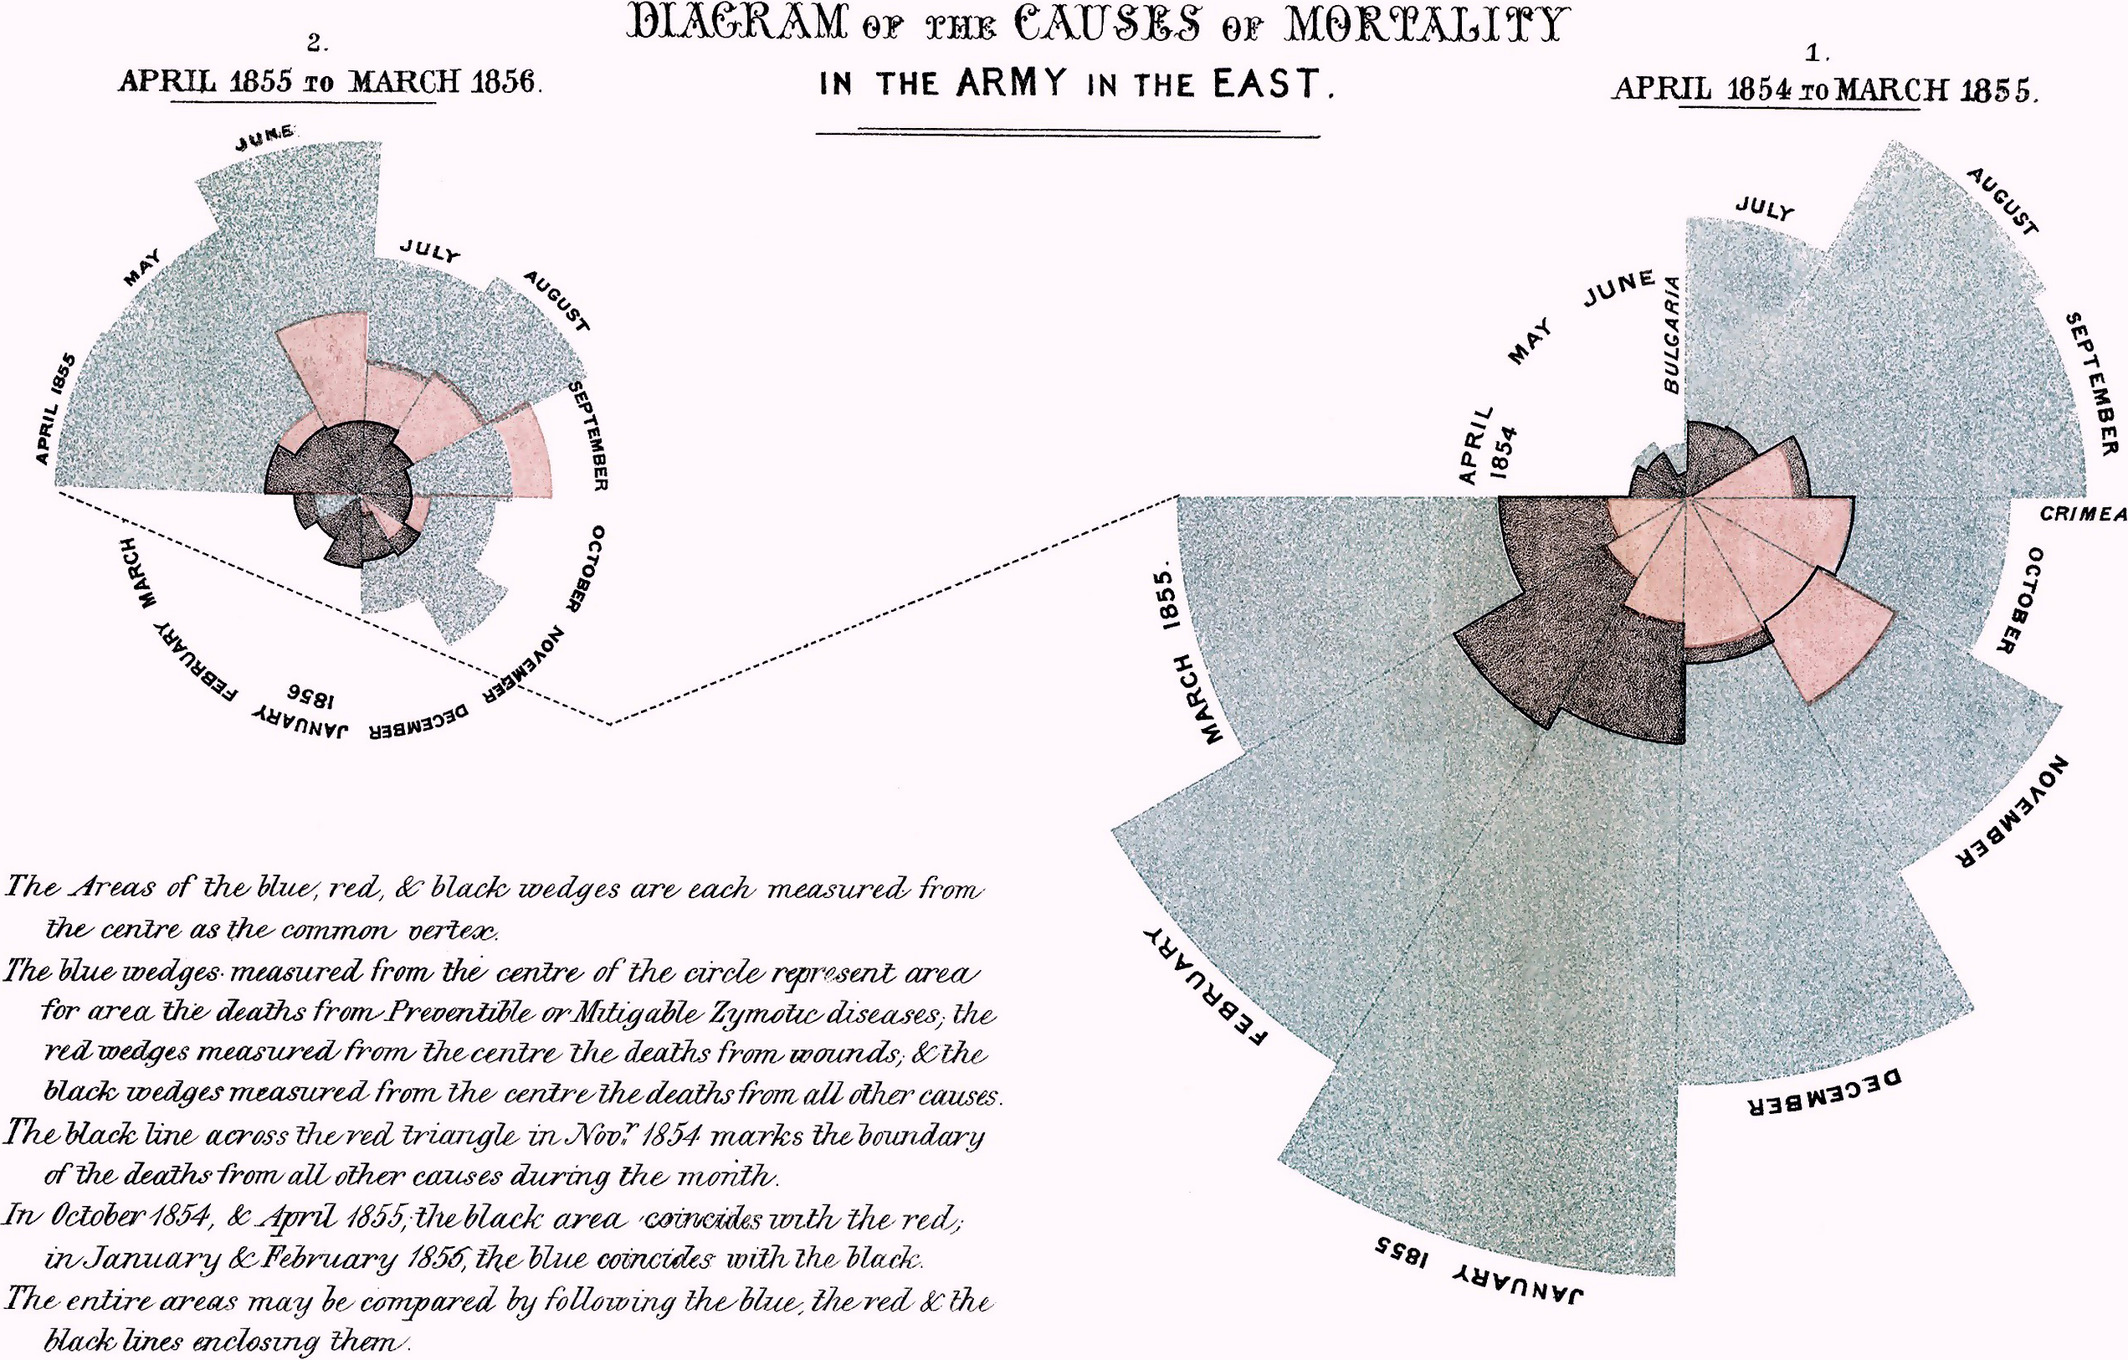
\includegraphics[width=\textwidth]{media/fig20.jpeg}
  \caption{Nightingale's coxcomb diagram on causes of mortality in the British army. Reproduced from O'connor \textit{et al} (2017)\cite{soa7}.}
  \label{fig:vsc}
\end{figure}


Today's healthcare industry, driven by data and evidence-based practice, continues to rely on the effective presentation of information. The plethora of digital health data from electronic medical records, telehealth systems, and wearable devices necessitates innovative visualization approaches to inform decisions and policies.

The science of data visualization has since matured, offering sophisticated representations of genomic, clinical, and personal health data to facilitate quick assimilation of information by diverse stakeholders. The legacy of Nightingale's pioneering spirit endures as the healthcare community leverages digital data and advanced visualization techniques to improve outcomes. Interdisciplinary initiatives that blend data visualization with machine learning address the challenges posed by the volume, variety, and interconnectedness of health data.

\subsection{Real World Evidence}\label{real-world-evidence}

Real-World Evidence (RWE) has emerged as a significant concept in healthcare, aiming to complement and extend the insights gained from Randomized Controlled Trials (RCTs). While RCTs are the gold standard for establishing causality and assessing the efficacy of new treatments under controlled conditions, they often do not reflect the full spectrum of patient profiles encountered in routine clinical practice. RWE seeks to fill this gap by analyzing the outcomes of treatments as they are used in everyday settings, encompassing a diverse population with varying genetic backgrounds, comorbidities, and concomitant medications \cite{soa1}. This approach aims to provide a more comprehensive understanding of how treatments perform in the real world, thereby addressing the efficacy-effectiveness gap noted by Eichler \textit{et al} (2017)\cite{soa2}.

Given the intricate nature of RWE and its divergence from the more controlled environment of RCTs, transparency in methodology and findings becomes paramount. RWE studies, by capturing a diverse array of patient experiences in routine clinical settings, bring forth a complex interplay of genetic backgrounds, comorbidities, and treatments. This diversity, while enriching the data, introduces challenges in statistical evaluation due to the presence of confounding factors and biases, necessitating sophisticated analysis techniques for accurate interpretation \cite{soa3}\cite{soa4}.

The need for transparency extends to the sharing of data and code, facilitating computational reproduction and peer validation. However, the use of routinely collected electronic healthcare data often restricts public sharing due to privacy and regulatory constraints. This limitation underscores the importance of detailed reporting in RWE studies, providing a clear and comprehensive account of methodologies, data handling, and analytical strategies employed. Such detailed documentation ensures that, even when data cannot be shared, the processes and conclusions remain open to scrutiny and understanding. \cite{soa5}\cite{soa6}.

Wang et al. (2021) advocate for the harmonization and standardization of RWE practices to foster reproducibility and reliability in the field. This includes developing templates for planning and reporting that reduce inconsistencies and elevate the quality of RWE research. By adhering to these structured approaches and emphasizing transparency, the field of RWE can continue to provide valuable, nuanced insights into healthcare practices and outcomes, bridging the gap between clinical research and everyday medical care. The complexity of RWE findings necessitates not just textual explanation but also extensive visualizations. These visual tools are essential for illustrating the nuances of sub-analyses, sensitivity analyses, and other supplementary investigations, often accumulating into a substantial part of the supplementary material. Through detailed tables, figures, and a multitude of visual representations, researchers can offer a more transparent and digestible overview of their findings, aiding in the comprehension and further investigation of the intricate data landscapes characteristic of RWE studies \cite{soa5}.

\subsection{Visualization for Electronic Health Records (EHR)}\label{visualization-for-electronic-health-records-ehr}

\subsection{Research Oriented Visualizations}\label{research-oriented-visualizations}


Most research found focuses on EHR visualizations as a component of EHR interfaces for example, mostly in the context of Supporting Clinical Decision in the context of healthcare providing. The creation o visualizations for research yeld much fewer results.


\subsection{Advances in Interactive and Real-Time Visualization}\label{advances-in-interactive-and-real-time-visualization}

\subsection{Challenges in Healthcare Data Visualization}\label{challenges-in-healthcare-data-visualization}


\subsubsection{Data Complexity and Heterogeneity}\label{data-complexity-and-heterogeneity}
\subsubsection{Privacy and Security in Health Data}\label{privacy-and-security-in-health-data}
\subsubsection{Scalability and Performance in Visualization Tools}\label{scalability-and-performance-in-visualization-tools}

\subsection{Comparative Analysis of Visualization Tools}\label{comparative-analysis-of-visualization-tools}
\subsubsection{Evaluation of Existing Solutions}\label{evaluation-of-existing-solutions}
\subsubsection{Gaps and Opportunities for Visual Viper}\label{gaps-and-opportunities-for-visual-viper}

\subsection{Future Directions in Healthcare Visualization}\label{future-directions-in-healthcare-visualization}
\subsubsection{Emerging Technologies and Approaches}\label{emerging-technologies-and-approaches}
\subsubsection{Anticipated Challenges and Solutions}\label{anticipated-challenges-and-solutions}
